\clearpage
\section{Homogeneous Coordinates} \label{sec:homogeneous}

\begin{definition}
    Given a point $[a_1, a_2, \cdots, a_n]^\T \in \Real^n$, it can be expressed in homogeneous coordinates as $[\lambda a_1, \lambda a_2, \cdots, \lambda a_n, \lambda]^\T \in \Real^{n+1}$, where $\lambda \neq 0$ is a constant scale factor.
\end{definition}
In other words, homogeneous coordinates are a mathematical representation that extends the Cartesian coordinate system by introducing an additional coordinate. Consider the point $[u, v]^\T$ in 2D Euclidean space. We can convert it to homogeneous coordinates by adding a new coordinate, represented by $\widetilde{w}$:
\begin{equation}
    \begin{bmatrix}
        u \\ v
    \end{bmatrix}
    \sim
    \begin{bmatrix}
        u\widetilde{w} \\ v\widetilde{w} \\ \widetilde{w}
    \end{bmatrix}
    \equiv
    \begin{bmatrix}
        \widetilde{u} \\ \widetilde{v} \\ \widetilde{w}
    \end{bmatrix}
\end{equation}

\begin{figure}[H]
    \centering
    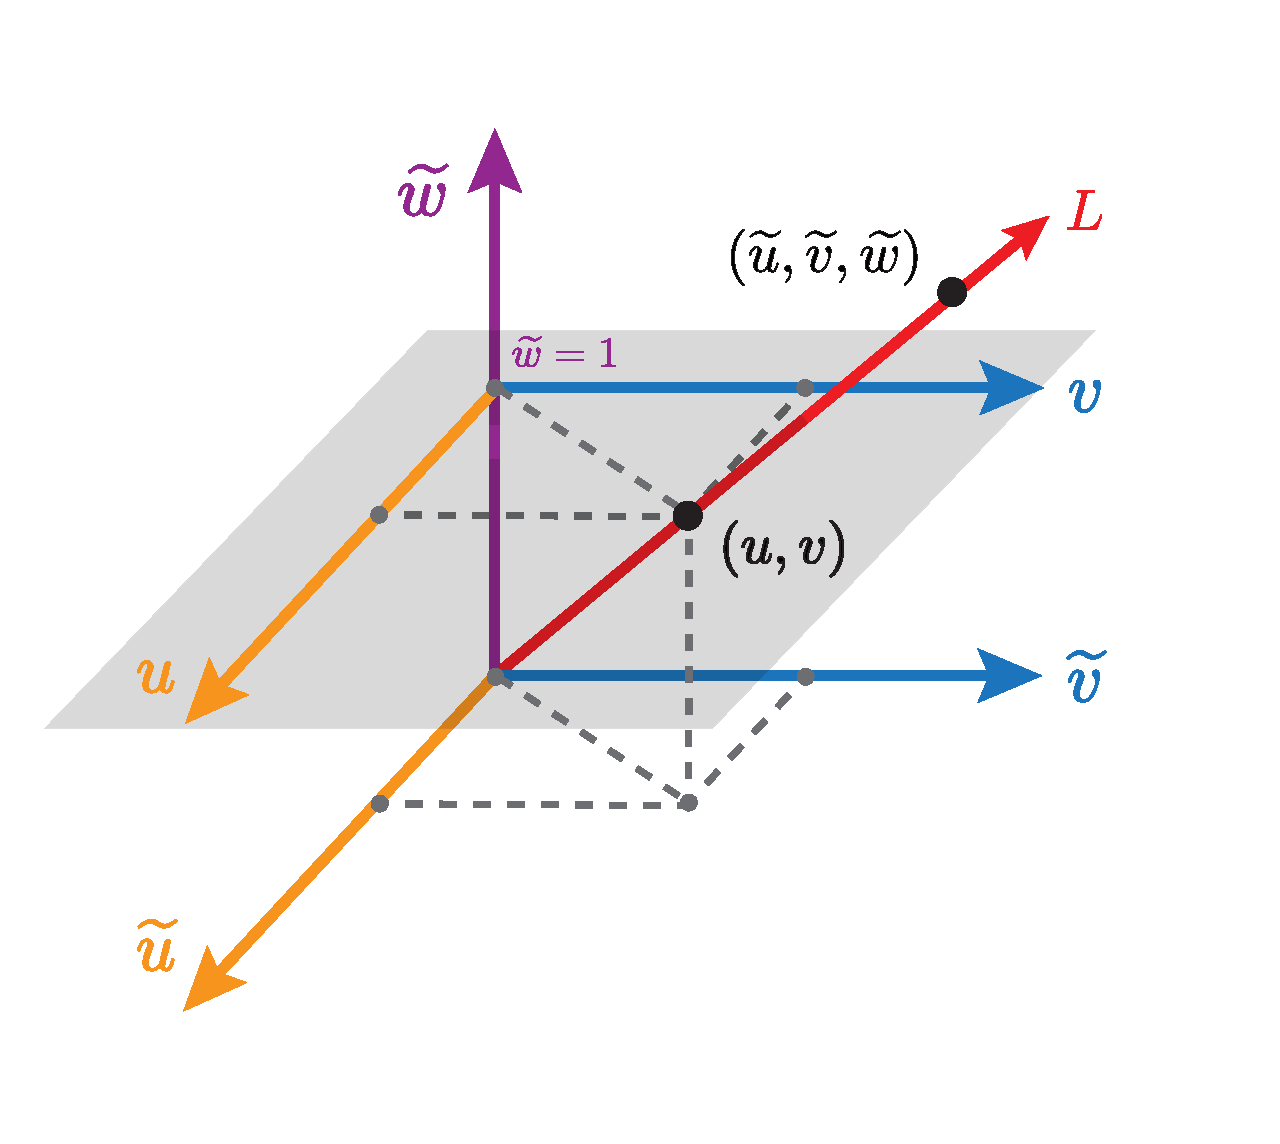
\includegraphics[width=0.6\textwidth]{diagrams/homogeneous}
    \caption{Homogeneous coordinate system.}\label{fig:homo}
\end{figure}

One important property of homogeneous coordinates is that if the homogeneous coordinate of a point is multiplied by a non-zero scalar, the result represents the same point, as visualized in Figure \ref{fig:homo}. For example, given the homogeneous point $[\widetilde{u},\widetilde{v},\widetilde{w}]^\T$:
\begin{equation}
    \begin{bmatrix}
        \widetilde{u} \\ \widetilde{v} \\ \widetilde{w}
    \end{bmatrix}
    \equiv
    k
    \begin{bmatrix}
        \widetilde{u} \\ \widetilde{v} \\ \widetilde{w}
    \end{bmatrix}
    \eqrestriction{k \neq 0}
\end{equation}
For this reason, homogeneous coordinates are able to simplify and generalize transformations, like translation, rotation, scaling, and perspective projection without the need for separate and complex formulas for each operation.






